{A water tank has the shape of an inverted pyramid, with dimensions given below, and is filled with water with a mass density of 1000 kg/m$^3$. Find the work performed in pumping all water to a point 5 m above the top of the tank.

\hfill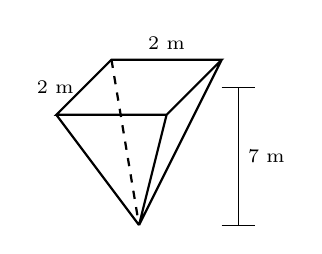
\begin{tikzpicture}[xscale=.7,yscale=.7]
\draw [thick] (0,0) -- node [pos=.5,left]{\scriptsize 2 m} (1,1) --node [above,pos=.5] {\scriptsize 2 m} (3,1) -- (2,0)--cycle
							(0,0) -- (1.5,-2)
							(3,1) -- (1.5,-2)
							(2,0) -- (1.5,-2);
\draw [thick,dashed] (1,1) -- (1.5,-2);
\draw (3,.5) -- (3.6,.5)
			(3,-2) -- (3.6,-2)
			(3.3,.5) -- node [pos=.5,right] {\scriptsize 7 m} (3.3,-2);
\end{tikzpicture}
\hfill\null
}
{617,400 j
}
